\documentclass{article}

% Language setting
% Replace `english' with e.g. `spanish' to change the document language
\usepackage[english]{babel}

% Set page size and margins
% Replace `letterpaper' with`a4paper' for UK/EU standard size
\usepackage[letterpaper,top=2cm,bottom=2cm,left=3cm,right=3cm,marginparwidth=1.75cm]{geometry}

% Useful packages
\usepackage{amsmath}
\usepackage{graphicx}
\usepackage[colorlinks=true, allcolors=blue]{hyperref}

\title{BDSA - Assignment 00}
\author{Mie Milvang-Jensen (MILV)}

\begin{document}
\maketitle


\section{Exercise 5 - description}

\textbf{Exercise 5 - Leap year function}.

A leap year in the Gregorian calendar is defined by the following rules (simplified):
Every year that is exactly divisible by four is a leap year, except for years that are exactly divisible by 100, but these centurial years are leap years if they are exactly divisible by 400. For example, the years 1700, 1800, and 1900 are not leap years, but the years 1600 and 2000 are.

Your function should have the following signature:

\begin{verbatim}
bool IsLeapYear(int year)
\end{verbatim}

Implement the function interatively using Test-Driven Development where first write a set of tests for the first rule (divisible by four) and then implement the rule.

\section{My Solution}
I have made a function based on the task given en exercise 5. The function takes an int (representing a year) as a parameter. At first the function checks if the year given is 1582 or after, if it is not, the function will throw a new Argument Exception. It then checks for the case that the given year is divisible by 100 but also by 400. In that case the given year is a leap the and the function returns true. If that is not true the functions checks if the given year is divisible by 100 but not by 400. In that case the given year is not a leap year and the function returns false. If that is also not true the function checks if the given year is divisible by 4. Since it has already checked for special cases at that point all other years that satisfies the statement is a leap year and the function will return true. If the statement isn't true the given year is not a leap year and the function returns false. 


\begin{figure}
\centering
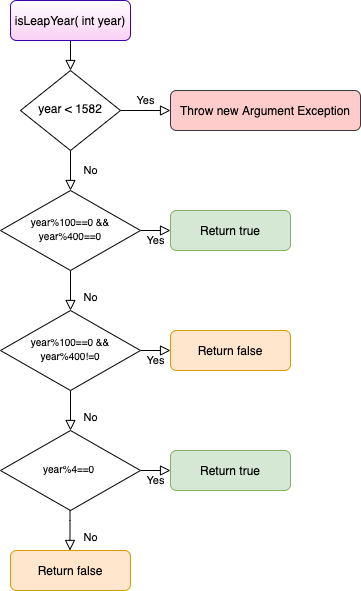
\includegraphics[width=0.6\textwidth]{isleapyearFigure.png}
\end{figure}



\end{document}